\documentclass[a4paper,14pt]{extarticle}

\usepackage[T2A]{fontenc}
\usepackage[utf8]{inputenc}
\usepackage[english,russian]{babel}
\usepackage[left=3cm, right=1.5cm, top=2cm, bottom=2cm]{geometry}

\usepackage{setspace}
\onehalfspacing{}

\usepackage[center]{titlesec}

\usepackage{indentfirst}
\setlength{\parindent}{20pt}

\usepackage{fancyhdr}
\setlength{\headheight}{17.0pt}
\pagestyle{fancy}
\fancyhf{}
\fancyhead[C]{\thepage}
\renewcommand{\headrulewidth}{0pt}

\usepackage[normalem]{ulem}

\hyphenpenalty=0

\usepackage[acronym]{glossaries}
\usepackage{multirow}
\usepackage[hidelinks]{hyperref}

\usepackage{graphicx}
\graphicspath{{images/}}

\usepackage{miller}
\newcommand{\unit}[1]{ \ \text{#1}}
\newcommand{\degree}{^\circ}
\newcommand{\celcius}{^\circ \text{C}}
\newcommand{\YEu}{${(\text{Y}_{1-x}\text{Eu}_x)}_2\text{O}_3$}
\newcommand{\range}[2]{[#1\div#2]}

\usepackage{forloop}
\newcounter{x}
\newcommand{\Repeat}[2]{\forloop{x}{0}{\value{x} < #1}{#2}}
\newcommand{\writedate}{<<\Repeat{2}{\ldots}>>\Repeat{5}{\ldots}2025г.}

\usepackage{csquotes}
\bibliographystyle{gost-numeric.bbx}
\usepackage[backend=biber,
citestyle=gost-numeric,
bibstyle=gost-numeric,
sorting=none,
]{biblatex}
\addbibresource{bibliography.bib}

\begin{document}
\begin{titlepage}
\thispagestyle{empty}
\begin{spacing}{1.15}
\footnotesize
\begin{center}
    МИНИСТЕРСТВО НАУКИ И ВЫСШЕГО ОБРАЗОВАНИЯ РОССИЙСКОЙ ФЕДЕРАЦИИ
    \vspace{20pt}

    ФЕДЕРАЛЬНОЕ ГОСУДАРСТВЕННОЕ АВТОНОМНОЕ ОБРАЗОВАТЕЛЬНОЕ\\
    УЧРЕЖДЕНИЕ ВЫСШЕГО ОБРАЗОВАНИЯ
    \vspace{6pt}

    «НОВОСИБИРСКИЙ НАЦИОНАЛЬНЫЙ ИССЛЕДОВАТЕЛЬСКИЙ ГОСУДАРСТВЕННЫЙ УНИВЕРСИТЕТ» (НОВОСИБИРСКИЙ ГОСУДАРСТВЕННЫЙ УНИВЕРСИТЕТ, НГУ)
    \vspace{10pt}
\end{center}
Факультет \uline{\textbf{ФИЗИЧЕСКИЙ}}
\vspace{10pt}

\noindent
Кафедра \uline{\textbf{ФИЗИЧЕСКИХ МЕТОДОВ ИССЛЕДОВАНИЯ ТВЕРДОГО ТЕЛА}}
\vspace{8mm}

\noindent
Направление подготовки \uline{\textbf{03.03.02 ФИЗИКА}}
\vspace{10pt}

\noindent
Образовательная программа: \uline{\textbf{БАКАЛАВРИАТ}}
\vspace{8mm}
\begin{center}
    \textbf{ВЫПУСКНАЯ КВАЛИФИКАЦИОННАЯ РАБОТА}

    \textbf{(научно-исследовательский формат)}
    \vspace{8mm}

    \uline{\hfill Кудрявцева Артема Леонидовича \hfill}

    $_\text{(Фамилия, Имя, Отчество автора)}$
    \vspace{8mm}
\end{center}
Тема работы \uline{Разработка методики определения параметров элементарной ячейки монокристаллов на дифрактометре, оснащенном двумерным детектором\hfill}
\vfill

\noindent
\textbf{«К защите допущена»}

\noindent
Заведующий кафедрой \hfill \textbf{Научные руководители}
\vspace{10pt}

\noindent
д.~ф.-м.~н., профессор \hfill д.~ф.-м.~н., профессор
\vspace{10pt}

\noindent
г.~н.~с. ИК СО РАН \hfill г.~н.~с. ИНХ СО РАН
\vspace{10pt}

\noindent
Цыбуля~С.В./\writesign{}\hfill{}Громилов~С.А./\writesign{}

\noindent
$_\text{(фамилия И., О.) / (подпись, МП)}$ \hfill $_\text{(фамилия И., О.) / (подпись, МП)}$
\vspace{10pt}

\noindent
\writedate\hfill м.~н.~с. ИНХ СО РАН
\vspace{10pt}

\noindent
\hfill Серебренникова~П.С./\writesign{}

\noindent
\hfill $_\text{(фамилия И., О.) / (подпись, МП)}$
\vspace{10pt}

\noindent
\hfill\writedate{}
\vspace{8mm}

\hfill Дата защиты:\writedate{}
\vspace{8mm}

\begin{center}
    Новосибирск, 2025
\end{center}

\end{spacing}
\end{titlepage}
\tableofcontents
\section{Введение}

Точность измерения параметров элементарной ячейки (ПЭЯ) монокристаллов на дифрактометрах, оборудованных 2D-детекторами, обсуждается достаточно активно~\cite{Herbstein:2000,Waterman:2010,Dudka:2010,Henn:2019,Taylor:1986,Serebrennikova:2021}.
В работе~\cite{Dudka:2017} проблема сформулирована следующим образом: <<\ldotsпопытки получить воспроизводимые значения параметров элементарных ячеек монокристаллов при повторных исследованиях или исследовать зависимости этих параметров от температуры или давления могут привести к разочарованию>>.
К этому можно добавить, что это утверждение справедливо и при сопоставлении данных рентгеноструктурного анализа (РСтА) монокристаллов и дифрактометрии поликристаллов.
Трудно перечислить все подходы, предложенные для минимизации ошибок измерения ПЭЯ монокристаллов.
Среди последних обзоров на эту тему можно указать~\cite{Galdecka:2006,Lider:2020}.
Возможности методик с использованием внешнего или внутреннего эталонов на ряде примеров продемонстрированы в работах~\cite{Gromilov:2022,Panchenko:2022,Panchenko:2023,Serebrennikova:2023,Serebrennikova:2022}.
Особо следует отметить, что эти методики ориентированы на исследование малых монокристаллов (т.е. имеющих размер меньше первичного пучка), пригодных для проведения РСтА.
Пробоотбор подходящих для исследования образцов такой же, как и для РСтА --- требуется совершенный кристаллик с линейными размерами <0.1~мм.
Дополнительное требование --- наличие рефлексов с разрешенным дублетом, если оно выполняется, то при использовании рефлексов с $2\theta \approx 120\degree$ и гониометров с точностью $0.005\degree$ можно рассчитывать на измерение межплоскостных расстояний с относительной ошибкой не хуже $\Delta d / d = 5 \cdot 10^{-5}$.
Не во всех случаях использование внутреннего эталона удобно, т.к. требует дополнительных усилий при подготовке и определении ориентации одновременно обоих кристаллов, а также приводит к уменьшению интенсивности и взаимному экранированию~\cite{Serebrennikova:2022}.
Использование внешнего эталона обычно вызывает вопросы об эквивалентности установки образцов.
В этом плане развитие безэталонных методик имеет свои перспективы.

Классической безэталонной методикой измерения ПЭЯ является схема Бонда~\cite{Bond:1960}, в основе которой лежат два основных фактора – наличие точного гониометра (достаточно одноосного) и сориентированной определенным образом монокристаллической пластинки (см. рис.~\ref{fig:bond}а).
Методика хорошо себя проявила на малых кристаллах~\cite{Lisoivan:1988}, хотя при использовании одноосных гониометров в случае кристаллов средних и низших сингоний требуется переклейка кристалла.
Современные монокристальные дифрактометры оснащаются моторизированными гониометрами позволяющими поворачивать образец вокруг двух- или трех осей, что делает их подходящими для реализации схемы Бонда.
Причем эту схему можно реализовать как на больших ориентированных монокристаллических пластинах, так и на малых кристаллах.
Если при измерениях на больших кристаллах (см. рис.~\ref{fig:bond}а) угол $2\theta = \omega_+ - \omega_-$ свободен от ошибок, связанных со смещением образца с оси гониометра, то во втором необходимо учитывать возможное смещение, т.е. эксцентриситет.
Эксцентриситет зависит как от размера сферы сведения осей (\textit{sphere of confusion}), так и точности центрирования образца.
Подходы к экспериментальному учету эксцентриситета малых монокристаллов достаточно хорошо проработаны в литературе см., например,~\cite{Ponomarev:1969,King:1979}.

\begin{figure}[ht!]
    \centering
    \begin{subfigure}{0.5\textwidth}
    \centering
    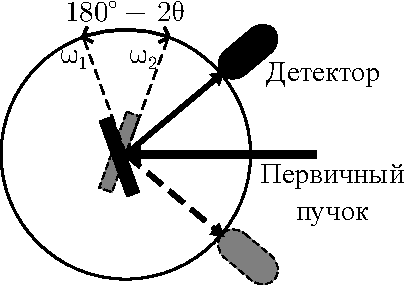
\includegraphics[]{bond.pdf}
    \caption{}%
    \label{fig:bond}
    \end{subfigure}%
    \begin{subfigure}{0.5\textwidth}
    \centering
    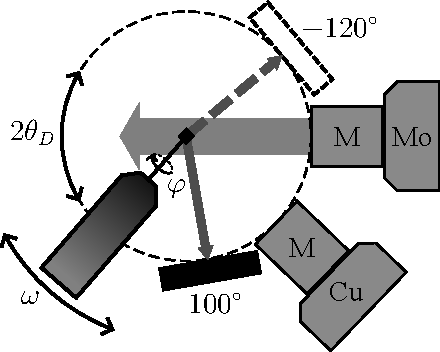
\includegraphics[]{our_bond.pdf}
    \caption{}%
    \label{fig:our_bond}
    \end{subfigure}
    \caption{Схемы эксперимента для учета эксцентриситета образца.}%
\end{figure}

Кроме этого, точность измерения ПЭЯ зависит от точности гониометра.
В паспорте сейчас обычно указывают лишь воспроизводимость установки углов, и не указывают значение самой погрешности.
Другие ошибки, возникающие при использовании серийных приборов, ориентированных на проведение РСтА, обусловлены значительной расходимостью первичного пучка (на уровне нескольких десятых градуса).
На точность измерений влияет и общая компоновка гониометра: при горизонтальном расположении рентгеновской трубки доступные для съемки углы $2\theta$ значительно ограничены.
Использование 2D-детектора также ограничивает углы $2\theta$, а также предполагает обработку двумерных профилей, что вносит свои нюансы в определение положения максимума, особенно при неполном разрешении дублета.
В основе точности измерений ПЭЯ в схеме Бонда лежит значение использованной длины волны, далее будут использованы рекомендованные значения $\lambda \text{Mo} K \alpha_1 = 0.70931715 (41)\unit{\AA}$ и $\lambda \text{Mo} K \alpha_2 = 0.713607 (12)\unit{\AA}$~\cite{Deslattes:1985}.

Проведение измерений ПЭЯ с максимально достижимой точностью всегда было особым разделом рентгенографии.
Уже для первых дифрактометров был предложен ряд подходов к учету основных приборных ошибок~\cite{Ponomarev:1969}. В~\cite{King:1979} предложен метод учета основных ошибок по результатам съемки 8 рефлексов на приборе, оснащенном четырехкружным гониометром и точечным детектором.
Цель настоящей работы --- оценка и учет ошибок измерений ПЭЯ, связанных с эксцентриситетом образца, в схеме Бонда на современных дифрактометрах.
Для этого логично привлечь эталонные образцы, для которых ПЭЯ известны с хорошей точностью.

\section{Обзор методов}

Перед разработкой самой методики были изучены обзорные статьи~\cite{Lider:2020,Galdecka:2006} с целью поиска базового метода, на котором можно будет построить желаемую методику.
В указанных обзорах приводятся различные рентгеновские дифракционные методы измерения и уточнения ПЭЯ.
Их все можно разбить на три группы:
\begin{itemize}
    \item Полихроматические методы (метод Лауэ)
    \item Методы с монохроматичным, но широко расходящимся пучком (метод косселевских проекций)
    \item Методы с монохроматичным и коллимированным пучком.
\end{itemize}
Среди них выбирался тот, который можно адаптировать под стандартный лабораторный монокристальный дифрактометр.
Такой дифрактометр предполагается оснащенным:
\begin{itemize}
    \item Рентгеновской трубкой с хорошо коллимированным пучком
    \item Как минимум однокружным гониометром для образца
    \item Матричным детектором с регулируемым углом поворота вокруг образца
\end{itemize}
Таким образом, в рассмотрении остаются только методы, использующие монохроматическое и коллимированное излучение, так как используемое в лабораторных дифрактометрах характеристическое излучение можно считать монохроматическим, относительно фонового тормозного.

\subsection{Метод Бонда}

В первую очередь из этих методов выделяется метод Бонда.
Он является простым, безэталонным, универсальным, и позволяющим получить хорошую точность, вплоть до $10^{-6}$.

В оригинальном исполнении схема Бонда~\cite{Bond:1960} представляет собой однокристальный спектрометр.
В качестве источника используется микрофокусная рентгеновская трубка с коллиматором в виде пары пластин дающих расходимость первичного пучка около $0.8'$.
Кристалл --- это ориентированная полированная пластина из монокристаллического кремния, значительно превосходящая размерами первичный пучок.
Для поддержания постоянной температуры в $24.7\celcius$ образца при этом используется водяное охлаждение.
Кристалл был закреплен на гониометре, позволяющим регулировать угол наклона кристалла и вращать его в одной плоскости $\omega$ с точностью до $1''$.
В качестве детекторов использовались два счетчика гейгера, которые считаются точечными детекторами.
Они могли вращаться в той же плоскости, что и кристалл.

Само измерение ПЭЯ в схеме Бонда выглядит так:
\begin{enumerate}
    \item Выбирается плоскость кристалла, отражение от которой будет измеряться
    \item Отражающая плоскость выставляется перпендикулярно первичному пучку
    \item Детектор устанавливается под углом, чтобы зарегистрировать отражение от плоскости
    \item Измеряется зависимость интенсивности на детекторе от угла поворота $\omega$ кристалла вблизи отражающего положения (кривая качания)
    \item Из полученной зависимости определяется угол $\omega_1$ при котором достигается максимум интенсивности на детекторе
    \item Предыдущие три шага повторяются для симметричного положения детектора и определяется второй угол $\omega_2$
    \item Угол дифракции вычисляется как $2\theta=180\degree-|\omega_1-\omega_2|$
\end{enumerate}
Затем уже значения межплоскостных расстояний вычисляются из уравнения Вульфа-Брэгга~(\ref{eq:bragg}), и, зная индексы Миллера отражающих плоскостей и сингонию кристалла, это позволяет вычислить наконец и значения ПЭЯ.

При определении угла $2\theta$ по такой схеме исключаются ошибки, связанные с:
\begin{itemize}
    \item Смещением образца (эксцентриситетом)
    \item Поглощением в кристалле
    \item Положением нуля гониометра
\end{itemize}
Другие же ошибки имеют незначительное влияние и для них есть выражения, позволяющие вводить поправки для их учета.
Список источников этих ошибок:
\begin{itemize}
    \item Неточное выведение отражающей плоскости параллельно оси вращения $\omega$
    \item Расходимость первичного пучка
    \item Отклонение первичного пучка от плоскости $\omega$
    \item Преломление в кристалле
    \item Фактор Лоренца-поляризации
    \item Ошибка измерения угла
\end{itemize}

В оригинальной работе Бонда ему удалось достигнуть относительной погрешности определения ПЭЯ около нескольких частей на миллион, то есть порядка $10^{-6}$.

\subsection{Модификации метода Бонда}

Схема Бонда была адаптирована и для изучения малых монокристаллов~\cite{Hubbard:1976,Ponomarev:1969}.
Для этого было предложено дополнительно измерять угол отражения от фриделевской пары выбранной плоскости.
Углы $\omega$ для фриделевской пары плоскостей отличаются в таком случае на $180\degree$, и это позволяет уменьшить ошибку калибровки гониометра.
Остальные ошибки уменьшаются за счет учета ассиметричности кривой качания.
Она смещает измеряемое значение угла $\omega$, но при использовании фриделевской пары, это смещение в оказывается преимущественно направлено в разные стороны.
Таким образом, полусумма углов $\omega$ для фриделевской пары плоскостей позволяет в среднем уменьшить погрешность определения ПЭЯ.

Для трехкружного гониометра возможно использование методики измерения от одной плоскости уже для 8 различных углов гониометра~\cite{King:1979}.
В такой схеме можно учесть еще больше ошибок, связанных со смещением образца от точки сведения осей гониометра, а также она позволяет определить нулевые положения гониометра.
Для реализации этого метода даже была написана специальная программа, которые позволяют калибровать дифрактометры с трехкружными гониометрами и точечными детекторами~\cite{Angel:2011}.

\subsection{Метод щелей Соллера}

В работе~\cite{Berger:1984} предлагается метод, использующий всего одно отражающее положение кристалла, но при этом получаемая точность оказывается не хуже чем в методе Бонда, то есть порядка $10^{-6}$.
Угол дифракции же в нем измеряется с помощью щелей Соллера.

В этом методе сначала кристалл и детектор выводятся в отражающее положение, при котором наблюдается максимальная интенсивность дифрагированного луча.
После этого на гониометр устанавливаются щели Соллера, и измеряется угол между их положениями на гониометре, в которых наблюдается максимальная интенсивность.

Из-за использования щелей Соллера, этот метод оказывается невосприимчивым к центрировке образца, и в нем можно использовать источник с большой расходимостью.
По сравнению с методом Бонда он оказывается более сложным, и требует больше специального оборудования для реализации.

\subsection{Метод четырехкристального спектрометра}

Похожий метод измерения угла~\cite{Fewster:1989} использует два кристалла для монохроматизации первичного пучка и один на дифрагированном пучке.
Этот метод, так же как и использующий щели Соллера, невосприимчив к центрировке образца.
Из его недостатков можно отметить, что он требует серьезной модификации установки и тщательной юстировки.

\subsection{Метод компланарных рефлексов}

Этот метод~\cite{Isomae:1976} возможен только для кристаллов, в которых угол между определенными плоскостями однозначно определяется индексами Миллера и не зависит от экспериментально определенных параметров.
При этом измеряется малый угол, на который нужно повернуть кристалл, чтобы вместо отражения от одной плоскости, появилось отражение от второй.
Из-за малого угла поворота, условия съемки практически неизменны для двух отражающих положений, что позволяет свести ошибки, связанные с этим к минимуму.
Этот метод также обладает высокой точностью, на уровне $10^{-6}$.

\subsection{Метод многолучевой дифракции}

Многолучевая дифракция возникает, когда две или более плоскостей оказываются в отражающем положении одновременно.
При этом возможно наблюдение рефлексов, запрещенных кинематической теорией дифракции.
Такое явление впервые наблюдалось Реннингером~\cite{Renninger:1937} и было названо им \textit{Umweganregung} или <<окольным возбуждением>>.
Пики, возникающие в при многолучевой дифракции, получаются более узкими, чем обычные, и поэтому их положение можно измерять более точно.
Но точность такого метода в итоге оказывается не сильно лучше того же метода Бонда: всего лишь на уровне $10^{-5} - 10^{-6}$.

\subsection{Методы эталонов}

Методы эталонов предполагают определение межплоскостных расстояний опираясь не на известную длину волны, а на хорошо известные ПЭЯ эталонного кристалла.
Вообще, эталоны могу использоваться неявно для калибровки дифрактометра, или явно в виде дополнительных, используемых одновременно с образцом кристаллов.
Может быть применен внутренний эталон как в порошковой дифракции, где в исследуемый образец добавляются кристаллы эталонного и снимается дифракционная картина их обоих одновременно.
Использование эталонов само по себе не является конкретной схемой эксперимента, а говорит о внедрении в него дополнительного источника информации.
Явное использование эталонов для измерения ПЭЯ никак не будет использоваться для разработки методики, так как это достаточно сложно и не подходит под поставленные условия.

\subsection{Выбор метода}

Среди всех перечисленных методов в итоге был выбран самый первый --- метод Бонда.
Его простота и универсальность оказываются очень привлекательными и поэтому должны сделать итоговую методику более доступной.
% \section{Теоретическая часть}

Главной особенностью современных дифракционных установок является, как уже было отмечено во введении, использование двумерных детекторов вместо точечных.
Поэтому классическое измерение угла $\omega$, при котором наблюдается максимум интенсивности дифрагированного луча оказывается крайне неэффективным.
Ведь при этом пришлось бы делать большое множество изображений с малым шагом, вычислять интегральную интенсивность луча, суммируя значения в определенной области детектора, а затем находить математическими методами угол, при котором и наблюдается максимум.
Такая схема проведения эксперимента является очень неэффективной и, в принципе, неестественной для современных дифрактометров, ведь сейчас обычно производится съемка при равномерно вращающемся кристалле в небольшом диапазоне углов, или, так называемое, сканирование.
Предлагается использовать именно результат такого сканирования для точного определения угла дифракции.

\subsection{Описание сканирования}

Рассмотрим идеализированную модель эксперимента, где пучок идеально коллимирован и монохроматичен, кристалл совершенен, а детектор позволяет абсолютно точно измерить интенсивность падающего на него излучения в каждой точке.
В таком случае, в кинематической теории дифракции, отражение от выбранной плоскости кристалла будет наблюдаться может только при дискретном наборе углов сканирования $\omega$.
Дифрагированный пучок же будет иметь нулевую расходимость, как и первичный.
Понять это можно, например, рассматривая уравнение Вульфа-Брэгга в более общем виде, чем~(\ref{eq:bragg}):
\begin{equation} \label{eq:bragg_general}
    \vec{k} + \vec{q} = k \vec{n}
\end{equation}
где $\vec{k}$ --- волновой вектор первичного пучка, $\vec{q}$ --- вектор рассеяния, равный по величине вектору обратной решетки выбранной плоскости, который вращается в процессе сканирования из-за вращения самого кристалла, $k$ --- длина вектора $\vec{k}$, а $\vec{n}$ --- единичный вектор направления дифрагированного луча.
В используемой модели вектор $\vec{k}$ является постоянным, а вектор $\vec{n}$ произвольным, так как двумерный детектор может регистрировать двумерное множество направлений $\vec{n}$.
Поэтому, можно возвести обе части векторного уравнения~(\ref{eq:bragg_general}) в квадрат и получить скаляры.
\begin{equation} \label{eq:squared_bragg}
    2(\vec{q}(\omega) \cdot \vec{k}) + q^2 = 0
\end{equation}
Теперь, так как сканирование производится вдоль одной оси, то вектор $\vec{q}$ зависит только от одной переменной --- угла сканирования, а значит решениями получившегося уравнения окажется дискретный набор углов.
В итоге картина интенсивности на детекторе при сканировании в области, захватывающей один угол $\omega$, при котором наблюдается отражение будет представлять собой просто дельта-функцию.

В реальности же, конечно, дельта-функция уширяется и представляет собой локализованный двумерный профиль в виде пика, или нескольких пиков (например, пары, при разделении дублета $K\alpha_{1,2}$).
Форма этого профиля определяется множеством различных факторов: спектром источника, структурой и формой кристалла, параметрами детектора, сканирования, и так далее.
Все это влияние принято учитывать в виде так называемой инструментальной функции.
Информация о ней позволяет из экспериментально полученных данных точно определить положение дифракционного профиля на детекторе, соответствующее идеализированной модели.
Но теоретическое вычисление инструментальной функции чаще всего или невозможно или очень трудоемко.
Поэтому можно либо измерять ее экспериментально, либо аппроксимировать эмпирически полученными функциями.

\subsection{Геометрия установки}

Чтобы более строго описать процесс измерения необходимо ввести набор понятий, которые определяют геометрию установки, и используются в работе в дальнейшем.

Уже была введена ось $\omega$, при вращении кристалла вокруг которой производится сканирование.
Ей же соответствует и одноименный угол.
Также в требованиях к установке было отмечено, что детектор должен быть установлен на гониометре, допускающем вращение вокруг образца.
Соответствующая плоскость вращения и одноименный с ней угол будут называться $2\theta_D$.
Ось вращения детектора названа так из-за того, что она юстируется специально, чтобы первичный пучок находился точно параллельно ей.
Угол $2\theta_D$ также для однозначности будем нормировать на интервал $(-180\degree, 180\degree)$.

Также необходимо ввести систему координат детектора.
Обычно она появляется естественным образом, так как детектор образует матрицу, и координатами в этом случае являются целочисленные индексы пикселей на ней.
Сейчас же введем координаты детектора $X$ и $Y$ таким образом, чтобы ось $X$ была параллельна плоскости $2\theta_D$, а ось $Y$ --- перпендикулярна ей.

\subsection{Схема Бонда}

Теперь, по аналогии со съемкой одного рефлекса в двух симметричных положениях в методе Бонда, проведем два $\omega$-сканирования для таких же симметричных положений.
Но в нашем случае, их логично расположить в плоскости $2\theta_D$, так как при полном  
% chktex-file 44
\section{Экспериментальная часть}
\subsection{Описание установки}
Рентгенографические эксперименты проводились на монокристальном дифрактометре Bruker D8 Venture (см. рисунок~\ref{fig:D8_photo}).
Его оборудование и характеристики:
\begin{itemize}
    \item Микрофокусная трубка Incoatec $I \mu S \ 3.0$
    \begin{itemize}
        \item $\text{Cu} K\alpha$ и $\text{Mo} K\alpha$ излучение
        \item Монохроматизация и коллимация с помощью многослойных зеркал Монтеля
        \item Диаметр пучка $110\unit{мкм}$
        \item Расходимость $0.3\degree$
    \end{itemize}
    \item Двумерный детектором PHOTON III
    \begin{itemize}
        \item CMOS-технология матрицы
        \item Разрешение $768 \times 1024$ пикселей
        \item Размер пикселя $135 \times 135\unit{мкм}^2$
        \item Ручная установка расстояния до образца
    \end{itemize}
    \item Трехкружный гониометр FIXED-CHI
    \begin{itemize}
        \item Гониометр использует эйлерову геометрию
        \item Автоматическая регулировка углов $\varphi$ и $\omega$ для образца и $2\theta_D$ для детектора
        \item Угол $\chi$ фиксирован и равен $54.7112\degree$
        \item Воспроизводимость установки углов $0.0001\degree$
        \item Точность установки углов $0.004\degree$\footnote{Паспортная точность установки углов не указана, но согласно результатам измерения эталонного образца на порошковом дифрактометре Bruker D8 Advance, оснащенном аналогичным гониометром, она не хуже $0.005\degree$.}
    \end{itemize}
    \item Температурная приставка Oxford Cryostream 800Plus
    \begin{itemize}
            \item Стабильность поддержания температуры $0.2\unit{К}$
    \end{itemize}
    \item Управление прибором средствами программного пакета APEX3~\cite{Bruker:2019}
\end{itemize}

\begin{figure}[ht!]
    \centering
    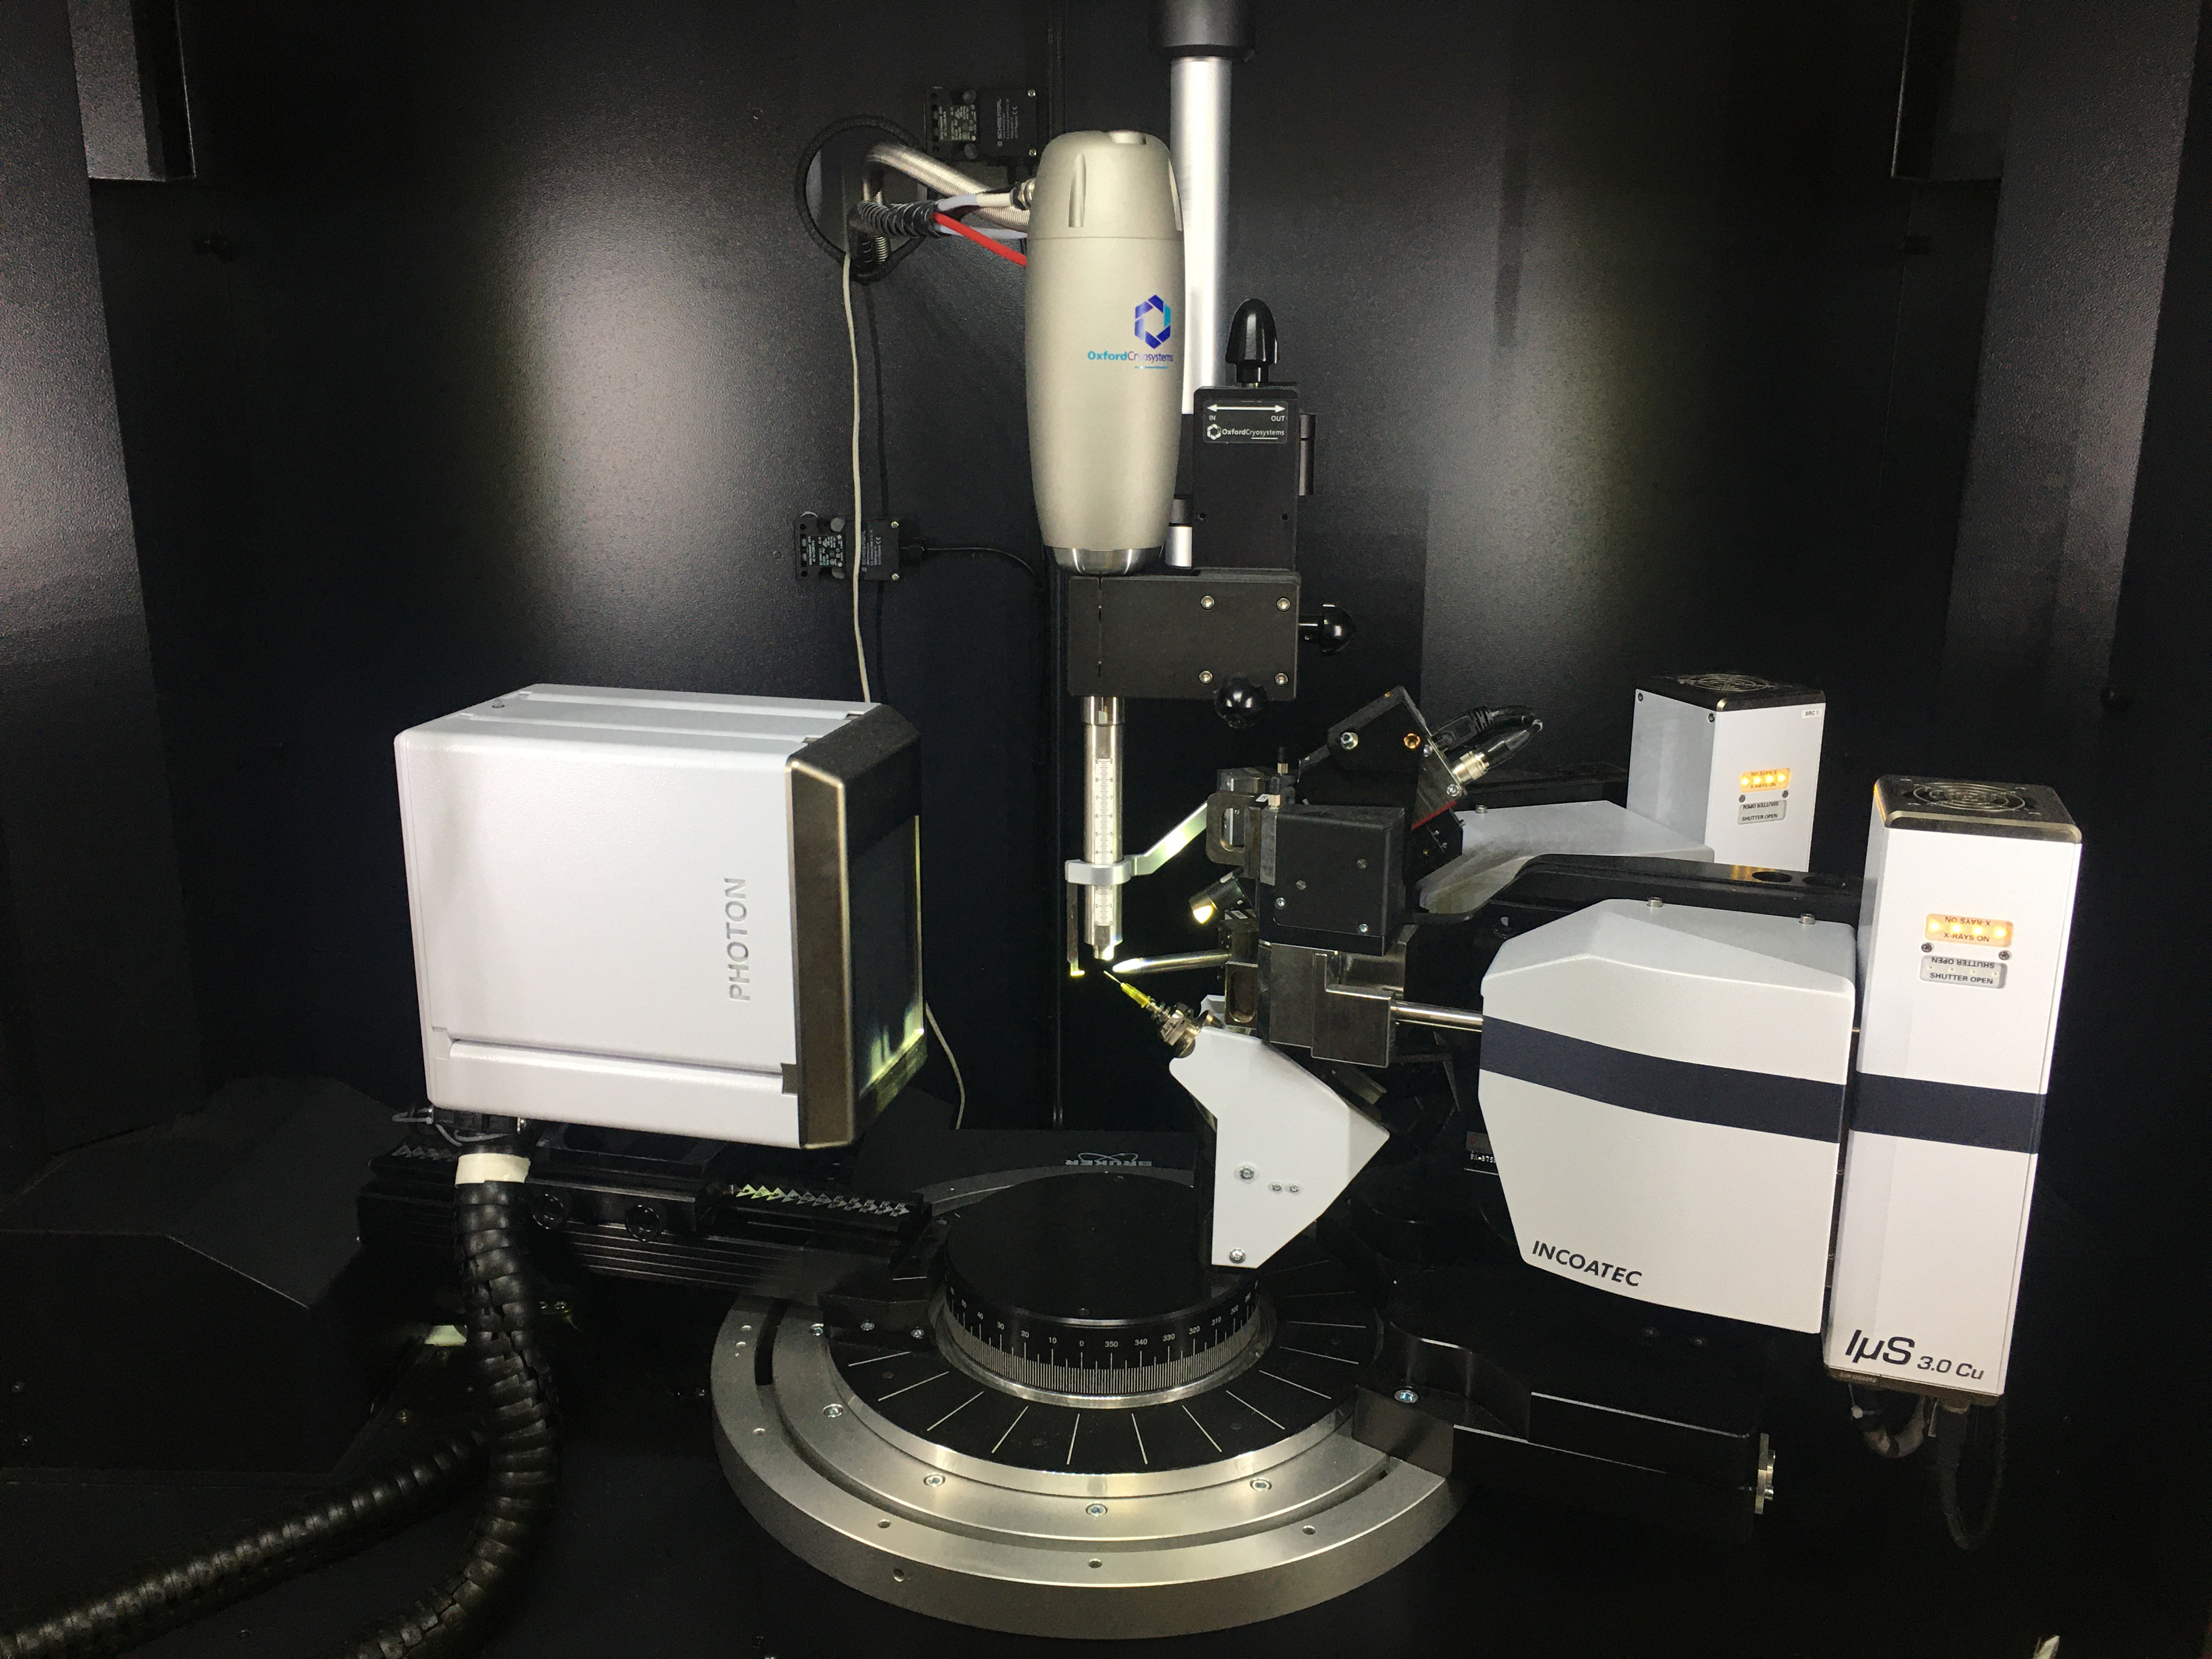
\includegraphics[width=0.8\textwidth]{d8_3.jpeg}
    \caption{Фотография установки}%
    \label{fig:D8_photo}
\end{figure}

\subsection{Исследуемые образцы}

Все изученные монокристаллы имели линейные размеры $\approx50\unit{мкм}$.
Монокристалл Si являлся осколком кристалла, который ранее был исследован на однокристальном спектрометре: $a_\text{Si} = 5.430933 (12)\unit{\AA}$~\cite{Lisoivan:1982}.
Однако, надо учесть, что это значение было вычислено исходя из $\lambda \text{Cu} K\alpha_1 = 1.540562\unit{\AA}$.
При использовании рекомендованной в настоящее время длины волны $\lambda \text{Cu} K\alpha_1 = 1.5405929\unit{\AA}$~\cite{Holzer:1997}, $a_\text{Si} = 5.431042(12)\unit{\AA}$.
Кристалл был смонтирован на гониометрической головке и тщательно сцентрирован (с поворотами по $\omega$ на $\pm 90\degree$). Для определения ориентации кристалла были проведены съемки трех серий $\varphi$-сканов шириной $0.5\degree$ при положениях детектора $2\theta_D = 0, \pm 45\degree$ (D = 70~мм).
Обработку фреймов проводили средствами APEX3 (процедуры: harvest, indexing, refinement), в результате был получен р4р-файл, содержащий информацию об ориентации кристалла относительно осей гониометра.
Аналогичная процедура была проведена с монокристаллом Ge.
Его ПЭЯ уточняли несколько раз методами однокристального спектрометра, многократных отражений и многолучевой дифракции: сводка данных приведена в~\cite{Lisoivan:1982}.
Значения $a_\text{Ge}$ лежат в интервале от $5.65776(2)\unit{\AA}$ до $5.657837(15)\unit{\AA}$, среднее значение $5.65779\unit{\AA}$ наиболее близко к $5.657772(10)\unit{\AA}$ [22].
Пересчет с использованием рекомендованного значения $\lambda \text{Cu} K\alpha_1 = 1.5405929\unit{\AA}$ приводит к $a_\text{Ge} = 5.657885\unit{\AA}$.

Монокристаллы \YEu{} получены методом роста из раствор-рас\-плава.
Продукт синтеза представлял собой мелкокристаллический порошок с размерами кристаллов от 0.2 до 1~мм.
Для исследования было отобрано 5 кристаллов с линейными размерами 20--40~мкм.

\subsection{Измерения в схеме Бонда}

Принципиальная схема эксперимента проведенного в схеме Бонда представлена на рис.~\ref{fig:bond}б.
В нашем случае наличие второго источника рентгеновского излучения ограничивает область доступных углов $2\theta_D$ значениями $\pm 97.5\degree$ (для $D = 128.5\unit{мм}$).
Второе ограничение связано со значительными геометрическими размерами детектора, что не дает блоку с установленной гониометрической головкой размещаться в определенных угловых интервалах.
По полученным р4р-файлам вычисляли углы $\varphi$ и $\omega$ для выведения рефлексов в отражающее положение на экваториальную плоскость.
Съемку рефлексов проводили в режиме $\omega$-сканирования угловых интервалов $\pm 2\degree$ относительно вычисленных значений $\omega$.
Такой интервал позволял зарегистрировать дублет полностью.
При съемке детектор устанавливали под углом $2\theta_D \approx 2\theta_{hkl}$, что обеспечивало регистрацию выбранного рефлекса центральной областью детектора.
Подробно методика описана в~\cite{Kudryavtsev:2024:YEu}.
Методику можно разделить на несколько этапов.

На первом этапе определяли ориентацию монокристалла относительно осей гониометра.
Такая съемка позволяет зарегистрировать существенную часть обратного пространства и провести качественное уточнение элементов матрицы ориентации для последующего вывода выбираемых рефлексов точно в отражающее положение на экваториальную окружность гониометра.
Кроме того, захват области дальних углов необходим для определения условий разрешения дублета $K\alpha$ и выяснения возможности уточнения ПЭЯ.
Обработку полученной серии фреймов проводили по программе APEX3.
В результате определяли предварительные значения ПЭЯ, дифракционный класс и ориентацию кристалла относительно осей гониометра (р4р-файл).
Этот этап соответствует первому этапу проведения РСтА.

Цель второго этапа --- поиск рефлексов, подходящих для измерения $d_{hkl}$.
В первую очередь мы рассматривали рефлексы с угловыми положениями $2\theta$ в узком интервале $\range{95\degree}{98\degree}$.
В случае эталонных монокристаллов (Si и Ge) структура известна, поэтому подходящие рефлексы были выбраны по теоретической дифрактограмме.
В общем случае, т.е. при неизвестной структуре, можно ориентироваться на предварительные значения ПЭЯ и дифракционный класс, установленный на первом этапе.
В случае Si и Ge для измерения ПЭЯ достаточно одного рефлекса, но для оценки уровня случайных ошибок взято большее количество.
Для поиска индексов кристаллографических плоскостей \hkl(h k l), которые могут быть выведены в отражающие положения при двух углах поворота детектора $2\theta_D$, была написана оригинальная программа James (язык Julia), доступная по ссылке https://github.com/m410y/James.jl.
Программа James использует информацию о текущей ориентации кристалла (р4р-файл) и вычисляет углы съемки $\varphi$ и $\omega$, при этом учитывая, что для записи рефлекса необходимо провести $\omega$-сканирование интервала $3-4\degree$.
Кроме этого, учитывается, что вывод в отражающее положение кристаллографической плоскости $(h k l)$, возможен при двух значениях $\omega$, число возможных ориентаций увеличивается вдвое (см. последний столбец табл. 1 Приложения).
Дополнительно программа сигнализирует о случаях, когда может быть использована и фриделевская пара \hkl(-h -k -l).
Съемка фриделевской пары позволяет по разнице значений координат $Y$ максимумов контролировать точность выведения рефлексов на экваториальную плоскость.
Некоторые дополнительные возможности программы James будут описаны далее.

На третьем этапе определяли общие условия проведения $\omega$-сканирования.
Для уменьшения ошибок, связанных с наклонами детектора, положение детектора задавали как $2\theta_D \approx 2\theta_{hkl}$.
При таком положении рефлекс фиксируется центральной областью детектора.
При выборе времени экспозиции ориентировались на получение интенсивности $K\alpha_1$-составляющей в максимуме $2 \cdot 10^4$ импульсов над фоном.
Время накопления фрейма в программе управления Bruker D8 Venture ограничено 10~мин, поэтому при необходимости, для достижения нужного уровня интенсивности, проводили несколько повторных съемок и далее суммировали фреймы средствами программы James. 
На четвертом этапе определяли координаты максимумов средствами программ Origin и James. Установлено, что результаты не отличаются.
Далее вычисляли разницу координат $X$ для двух симметричных положений детектора.
При переходе к углам дифракции рассчитывали угловые размеры пикселя $\gamma$, исходя из физических размеров пикселя ($135.3\unit{мкм}$) и выбранного $D$.
Контроль корректности такого расчета проводили по положениям $K\alpha_{1,2}$ составляющих согласно~\cite{Gromilov:2022}. 
Значение $2\theta_{hkl}$ вычисляли по формуле:
\begin{equation}\label{eq:bond2}
    2\theta_{hkl} = 2\theta_D + \gamma (X_- - X_+) / 2.
\end{equation}
При переходе к межплоскостному расстоянию $d$ использовали эталонное значение длины волны $\lambda \text{Cu} K\alpha_1 = 0.70931715(41)\unit{\AA}$.
Параметр элементарной кубической ячейки вычисляли по известной квадратичной форме: $1/d^2 = (h^2 + k^2 +l^2)/a^2$.

\section{Обсуждение результатов}
\subsection{Изучение Si}
Измерение проводилось в нескольких переустановках образца и разных расстояниях $D$ и углах $2\theta_D$.
Также для оценки возможности использования рефлексов отстоящих от центра детектора съемка фриделевской пары $\hkl(-9 7 1)/\hkl(9 -7 -1)$ была проведена при положении детектора $2\theta_D = \pm 97.5\degree$, что является крайним положением для $D = 128.5\unit{мм}$, которое отличается от идеального почти на $0.8\degree$.
Исследование фриделевской пары $\hkl(3 -3 1)/\hkl(-3 3 -11)$ показало разницу координат $Y$ всего 4 пикселя.
Среднее значение отклонение экспериментально полученных значений $2\theta$ от эталонных составило $0.0003\degree$, а среднее значение ПЭЯ отличается от эталонного на $0.0001\unit{\AA}$.
Относительная погрешность определения $d$ и ПЭЯ составила $5 \times 10^{-5}$.
\subsection{Изучение Ge}
На монокристалле Ge проводили контроль воспроизводимости установки образца и детектора.
Для этого было выполнено несколько переустановок образца, в том числе с коррекцией ориентации кристалла, изменением $D$ и угла $2\theta_D$.
При $D = 138.6\unit{мм}$ изучены рефлексы $\hkl(5 -11 -1)$ и $\hkl(1 -11 -5)$ с существенно отличными углами выведения в отражающее положение $(\varphi, \omega)$.
Для оценки возможности использования рефлексов, значительно отстоящих от центра детектора, съемка рефлекса $\hkl(7 -7 -7)$ была проведена при двух разных значениях $2\theta_D$.
Причем положение $\pm 99.9\degree$ отличалось от идеального почти на $1\degree$.
Исследование фриделевской пары $\hkl(3 -3 11)/\hkl(-3 3 -11)$ показало хороший уровень точности выведения рефлексов на экваториальную плоскость: разница координат $Y$ не превысила $\approx 7\unit{пикс.}$, что составляет $\approx 0.4\degree$.
В результате обработки профилей рефлексов были получены координаты максимумов и по формуле~\ref{eq:bond2} определены углы $2\theta$, а из них рассчитаны значения $d$ и ПЭЯ.
Среднее отклонение полученных значений $2\theta$ от теоретических составило $0.004\degree$, что соответствует точности гониометра.
Если ориентироваться на полученную величину, то относительная погрешность определения межплоскостного расстояния $\Delta d / d = 6 \times 10^{-5}$.
Таким образом, абсолютную погрешность определения ПЭЯ для Ge можно оценить как $0.0003\unit{\AA}$.
Среднее значение $a_\text{Ge} = 5.6579\unit{\AA}$ отличается от эталонного значения меньше, всего на $0.0001\unit{\AA}$.
\subsection{Изучение \YEu}
При выборе рефлекса, подходящего для уточнения ПЭЯ, мы столкнулись с проблемой оценки его интенсивности из-за хиральности точечной группы симметрии кристалла.
Так, например, теоретические значения структурной амплитуды рефлексов $\hkl(6 8 20)$ и $\hkl(8 6 20)$ соотносятся как 7 к 1.
Естественно, предпочтительно использовать наиболее интенсивное отражение.
Для решение этой проблемы предварительная съемка кристалла была скорректирована --- расстояние $D$ уменьшено до $60\unit{мм}$, а углы $2\theta_D$ увеличены до $\pm 75\degree$.
В результате были построены сечения обратного пространства, захватывающие область углов $2\theta = \range{95\degree}{100\degree}$.
Сопоставление интенсивностей рефлексов с результатами вычислений программы позволило выбрать оптимальные индексы.
По такой схеме было проведено исследование 5 монокристаллов.
Значения ПЭЯ лежат в интервале $\range{10.6902}{10.7045}\unit{\AA}$.
Разница крайних значений составляет $0.0143\unit{\AA}$.
Это значительно превосходит абсолютную погрешность определения ПЭЯ, равную $0.0007\unit{\AA}$.
Таким образом, можно однозначно утверждать, что синтезированный продукт не однороден.

Для оценки соотношения Y/Eu в изученных монокристаллах \YEu~можно использовать правило Вегарда.
Для построения соответствующей прямой были использованы литературные данные~\cite{Swanson:1954,Morris:1984}.

Для проведения РСтА расчет стратегии съемки для накопления полного массива данных производился для каждого кристалла автоматически с учетом его симметрии $(m\overline{3})$ по предварительно определенной матрице ориентации с использованием пакета программ APEX3.
Далее проводили интегрирование экспериментальных интенсивностей и вводили поправки на поглощение.
Структуры решены с помощью программы SHELXT~\cite{Sheldrick:2015:shelxt} и уточнены с SHELXL~\cite{Sheldrick:2015:shelxl} в графическом интерфейсе OLEX2~\cite{Dolomanov:2009}.
Параметры атомных смещений были уточнены в анизотропном приближении.

В результате установлено, что все изученные кристаллы изоструктурны и представляют собой твердые растворы \YEu, причем смешанными оказываются обе позиции металла.
\begin{figure}[ht!]
    \centering
    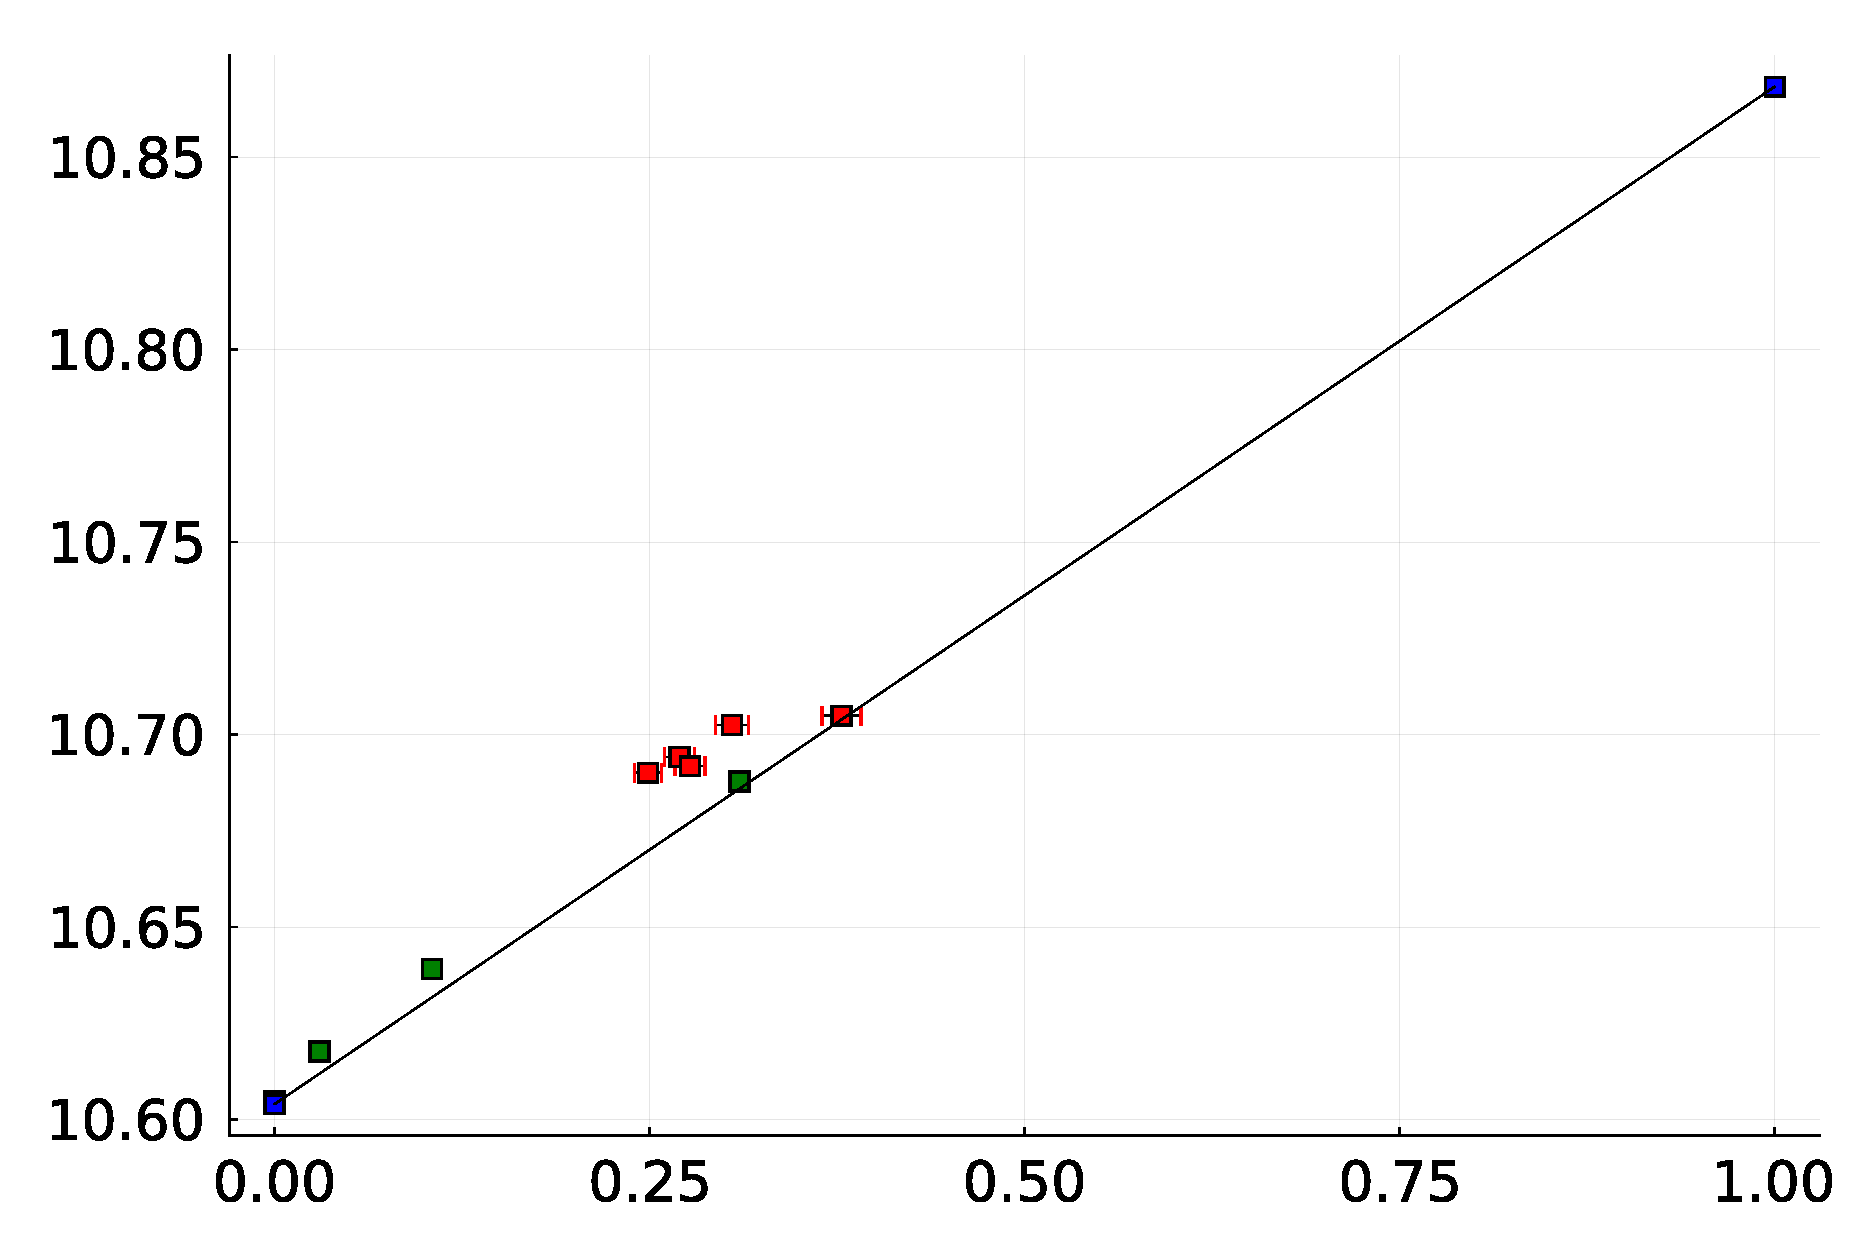
\includegraphics[width=0.8\textwidth]{YEu.pdf}
    \caption{Зависимость ПЭЯ \YEu~от мольной доли $x$.}
    \label{fig:YEu}
\end{figure}

\subsection{Оценка и учет эксцентриситета образца Si}
Несмотря на тщательную центрировку образца, в том числе с контрольными разворотами по оси $\omega$, крайне сложно точно определить его центр, особенно при неопределенной форме кристалла.
Можно ожидать, что при повороте вокруг оси $\omega$ центр образца движется по окружности, а сам образец описывает торообразную поверхность.
Подобную картину можно ожидать и при повороте образца вокруг оси $\varphi$.
Так как для использованного гониометра паспортное значение диаметра сферы сведения осей составляет $7\unit{мкм}$, центр образца при повороте вокруг обеих осей движется по достаточно сложной траектории.

Для оценки смещений центра образца при повороте вокруг оси $\varphi$, среди доступных для измерения рефлексов типов $\hkl{11 3 1}$, $\hkl{9 7 1}$ и $\hkl{9 5 5}$, было выбрано 10 вариантов, у которых значения $\omega$ лежат в интервале $\range{-82\degree}{95\degree}$.
Это примерно соответствует позиции образца при центрировании.
Все съемки проведены при одном положении детектора: $2\theta_D = -96.7\degree$, $D = 128.53\unit{мм}$.

Для оценки эксцентриситета при повороте вокруг оси $\omega$, были отобраны случаи, когда значения $\varphi$ лежат в интервале $\range{283.6\degree}{300.7\degree}$.
При этом соответствующие им углы $\omega$ лежат в интервале $\range{63.3\degree}{296.5\degree}$.
Область $\pm 60\degree$ недоступна из-за геометрических ограничений гониометра.
Графики зависимости координат от углов поворота представлены на графике~\ref{fig:eccentrSi}.

\begin{figure}[ht!]
    \centering
    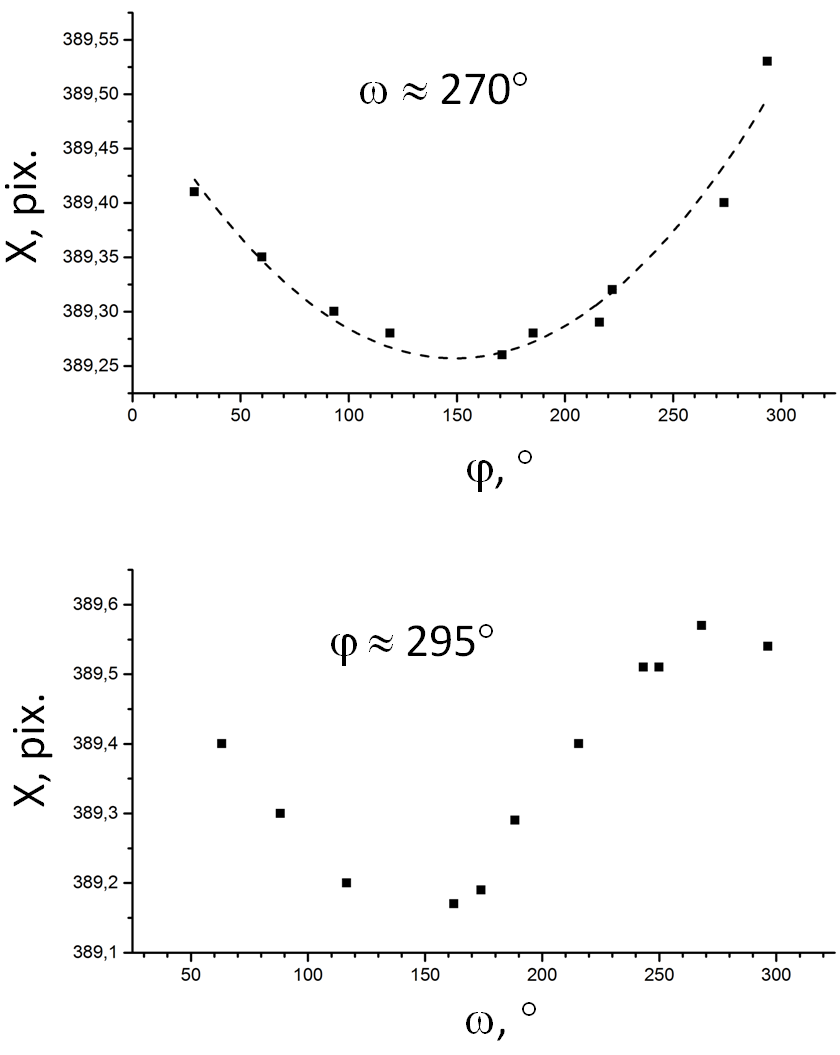
\includegraphics[width=0.8\textwidth]{eccentrSi.png}
    \caption{Смещение максимумов дифракционных отражений $\hkl(11 3 1)$, $\hkl(9 7 1)$ и $\hkl(9 5 5)$ по оси $X$ детектора из-за эксцентриситета образца: $a$ --– зависимость координаты $X$ от угла $\varphi$ (значения углов $\omega \approx 270\degree$); $b$ --- зависимость координаты $X$ от угла $\omega$ (значения углов $\varphi$ лежат в интервале от $\range{283.6\degree}{300.7\degree}$).}
    \label{fig:eccentrSi}
\end{figure}

Таким образом, проведенные два эксперимента показали одинаковую картину для эксцентриситетов, связанных с поворотами образца вокруг осей $\varphi$ и $\omega$.
При измерении ПЭЯ наиболее разумно исключить влияние именно последнего, тогда далее можно использовать подход, описанный выше~\cite{Ponomarev:1969}.

Среди всех вариантов рефлексов были выделены 5 фриделевских пар.
\subsection{Учет эксцентриситета для Si}
При произвольном выборе рефлексов расчет по~\ref{eq:bond2} приводит к значениям угла $2\theta$ в интервале $\range{96.722\degree}{96.747\degree}$.
Учет эксцентриситета по формуле~\ref{eq:bond4} уменьшает интервал значений до $\range{96.730\degree}{96.736\degree}$, а отклонения от теоретического значения не превышают $0.004\degree$.
Использование рефлексов с близкими значениями $\varphi = 66.31\degree, \, 59.35\degree$ позволяет пренебречь эксцентриситетом, связанным с поворотам вокруг оси $\varphi$.
Конечные результаты уточнения представлены в таблице~\ref{tab:Si:eccentr}.
\begin{table}[ht!]
    \centering
    \begin{tabular}{ |c|c| }
        \hline
        $2\theta$ & $96.732\degree$ \\
        $d$ & $0.47452 (3)\unit{\AA}$ \\
        $\Delta d / d$ & $6.2 \times 10^{-5}$ \\
        $a$ & $5.4311 (3)\unit{\AA}$ \\
        \hline
    \end{tabular}
    \caption{Результаты измерений ПЭЯ Si с учетом эксцентриситета.}
    \label{tab:Si:eccentr}
\end{table}

Можно отметить, что полученное значение ПЭЯ отклоняется от эталонного на $0.00006\unit{\AA}$.
Т. е. относительная разница составляет $1\times 10^{-5}$.
Еще раз подчеркнем, что результат получен лишь при частичном учете эксцентриситета, связанного с поворотом кристалла вокруг оси $\varphi$.
Чтобы полностью исключить такое влияние можно вывести одно из кристаллографических направлений вдоль оси $\omega$.
Тогда измерения можно проводить на рефлексах типа $hk0$.
При использовании трехкружного гониометра для образца такая проблема не возникает.
В нашем случае угол $\chi$ --- фиксирован, а штатные гониометрические головки предполагают только линейные смещения образца.
\subsection{Учет эксцентриситета для Ge}
Для устранения эксцентриситета, связанного с поворотом кристалла вокруг оси $\varphi$, монокристалл Ge был смонтирован на оригинальной гониометрической головке, имеющей возможность поворота образца вокруг одной оси на $\pm 10\degree$ (далее гониометрическая $\chi$--головка).
После определения ориентации кристалла были рассчитаны углы для выведения кристаллографического направления вдоль оси $\omega$. Алгоритм этого процесса описан в~\cite{Kudryavtsev:2024:eccentr}.

Расчеты для монокристалла Ge показали, что вдоль оси $\omega$ можно вывести направление $b$, так как для него значения угла $\chi = 2.2\degree$.
После поворота, исследование по нашей методике было проведено по рефлексам типа $\hkl{10 0 6}$.
Им соответствовало значение угла $2\theta = 93.943\degree$.
Все рефлексы регистрировались при одинаковых значениях угла $\varphi = -179.06\degree$.
Геометрические ограничения позволили отснять при $2\theta_D = \pm 93.9\degree$ только 12 из 16 теоретически возможных рефлексов.
При произвольных сочетаниях рефлексов значения $2\theta$, вычисленные по~\ref{eq:bond2} лежат в интервале $\range{93.935\degree}{93.958\degree}$.
Максимальные отклонения от теоретического значения достигают $0.015\degree$.
При использовании формулы~\ref{eq:bond4} углы $2\theta$ укладываются в интервал $\range{93.943\degree}{93.945\degree}$.
Отклонения от теоретического значения в таком случае не превышают $0.001\degree$.
Финальные значения для Ge представлены в таблице~\ref{tab:Ge:eccentr}.
Отклонение полученного значения ПЭЯ от теоретического составляет $0.0001\unit{\AA}$.
\begin{table}[ht!]
    \centering
    \begin{tabular}{ |c|c| }
        \hline
        $2\theta$ & $93.945\degree$ \\
        $d$ & $0.48515 (3)\unit{\AA}$ \\
        $\Delta d / d$ & $6.5 \times 10^{-5}$ \\
        $a$ & $5.6578 (4)\unit{\AA}$ \\
        \hline
    \end{tabular}
    \caption{Результаты измерений ПЭЯ Ge с учетом эксцентриситета.}
    \label{tab:Ge:eccentr}
\end{table}

Анализ координат $Y$ рефлексов Ge позволяет оценить точность выведения направления $b$ вдоль оси $\omega$.
Для этого можно построить зависимости $Y(\omega)$ для экспериментов, проведенных при дух симметричных положениях детектора $2\theta_D = \pm 93.9\degree$.
Она представлена на графике~\ref{fig:eccentrGe}.
В обоих случаях зависимости хорошо описываются синусоидами, но при $2\theta_D = -93.9\degree$ фаза сдвигается на $\theta$, а при $2\theta_D = +93.9\degree$ на $\theta + 180\degree$.
Для обработки всех рефлексов одновременно значения сдвигов вычитались из первичных значений $\omega$.
Из построенной аппроксимации следует, что максимальное отклонение направления $b$ от оси $\omega$ составляет $\approx 2.2\unit{пикс.}$, что эквивалентно $0.13\degree$.
Такое значение соответствует цене нониуса дуги гониометрической головки.
Так как отклонение лежит в ее плоскости, то можно утверждать что оно связано преимущественно с погрешностью установки угла $\chi$, а не $\varphi$.

\begin{figure}[ht!]
    \centering
    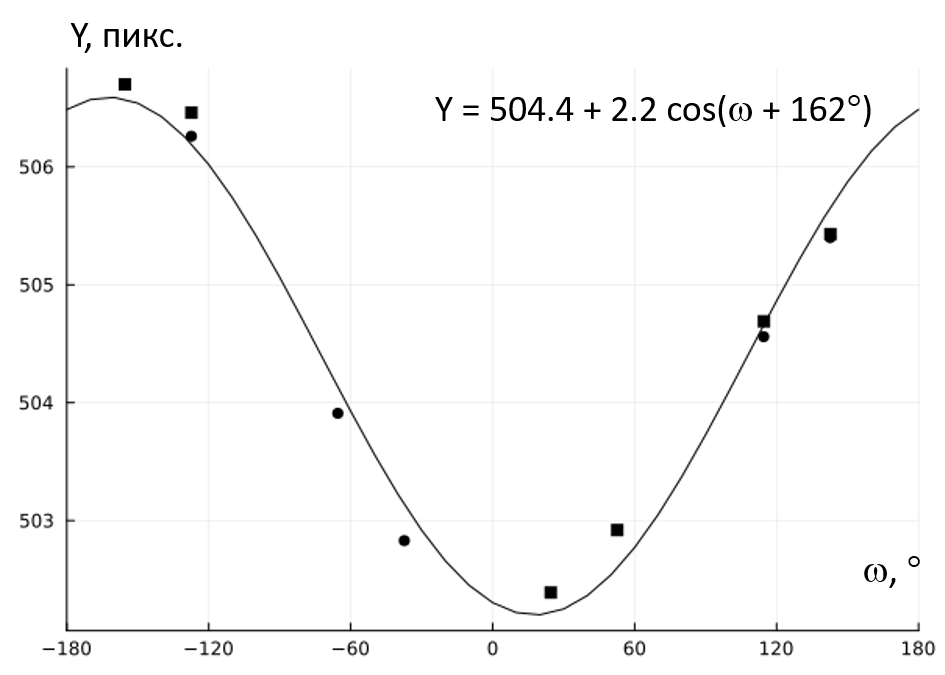
\includegraphics[width=0.8\textwidth]{eccentrGe.png}
    \caption{Зависимость координаты $Y$ от угла $\omega$ для монокристалла Ge. Для отрицательных (темные маркеры) и положительных (светлые маркеры) значениях $2\theta$ от значений $\omega$ были отняты значения $\theta + 90\degree$, тем самым позволив одновременно обработать все рефлексы. Аппроксимация функцией $Y = a_0 + a_1 \cos(\omega - \omega_1)$ выполнена с помощью МНК.}
    \label{fig:eccentrGe}
\end{figure}
\printbibliography{}
% chktex-file 44
\section*{Приложение}

\begin{table}[ht!]
    \centering
    \begin{tabular}{ |c|c|c|c|c|c| }
        \hline
                    $hkl$ &  $2\theta_D, \ \degree$ &     $\varphi, \ \degree$ & $\omega, \ \degree$ &    $Y,\unit{пикс.}$ &    $X,\unit{пикс.}$ \\
        \hline
        $  \hkl(11 -1 3)$ & \multirow{10}{*}{-96.7} &  \multirow{2}{*}{-66.31} &                88.2 &              504.77 &              389.27 \\
        $ \hkl(-11 1 -3)$ &                         &                          &               -91.8 &              503.78 &              389.53 \\
        $   \hkl(5 9 -5)$ &                         &   \multirow{2}{*}{28.72} &                84.7 &              505.36 &              389.40 \\
        $  \hkl(-5 -9 5)$ &                         &                          &               -95.3 &              503.24 &              389.41 \\
        $  \hkl(5 -9 -5)$ &                         &  \multirow{2}{*}{119.20} &               -99.5 &              501.71 &              389.28 \\
        $   \hkl(-5 9 5)$ &                         &                          &                80.5 &              506.90 &              389.58 \\
        $   \hkl(3 1 11)$ &                         & \multirow{2}{*}{-138.01} &                97.4 &              505.92 &              389.33 \\
        $\hkl(-3 -1 -11)$ &                         &                          &               -82.6 &              502.68 &              389.32 \\
        $  \hkl(3 -1 11)$ &                         & \multirow{2}{*}{-143.63} &                84.6 &              505.92 &              389.35 \\
        $ \hkl(-3 1 -11)$ &                         &                          &               -95.4 &              502.63 &              389.29 \\
        \hline
        $ \hkl(1 -3 -11)$ &  \multirow{10}{*}{96.7} &  \multirow{2}{*}{-59.35} &               -89.3 &              505.08 &              388.48 \\
        $  \hkl(-1 3 11)$ &                         &                          &                90.7 &              504.09 &              388.18 \\
        $   \hkl(9 -1 7)$ &                         &   \multirow{2}{*}{14.46} &                83.3 &              502.92 &              388.53 \\
        $  \hkl(-9 1 -7)$ &                         &                          &               -96.7 &              506.04 &              388.01 \\
        $   \hkl(9 5 -5)$ &                         &  \multirow{2}{*}{121.79} &                99.7 &              503.80 &              388.21 \\
        $  \hkl(-9 -5 5)$ &                         &                          &               -80.3 &              505.05 &              388.27 \\
        $  \hkl(-3 11 1)$ &                         & \multirow{2}{*}{-142.92} &                95.7 &              504.66 &              388.19 \\
        $ \hkl(3 -11 -1)$ &                         &                          &               -84.4 &              504.08 &              388.26 \\
        \hline
    \end{tabular}
    \caption{Положения пиков $K\alpha_1$ для эталона Si для $D = 128.5\unit{мм}$}%
    \label{tab:Si}
\end{table}

\begin{table}[ht!]
    \centering
    \begin{tabular}{ |c|c|c|c|c| }
        \hline
                   $hkl$ &  $2\theta_D, \ \degree$ & $\omega, \ \degree$ &    $Y,\unit{пикс.}$ &    $X,\unit{пикс.}$ \\
        \hline
        $ \hkl(-6 0 10)$ &  \multirow{6}{*}{-93.9} &              -112.4 &              503.91 &              388.61 \\
        $ \hkl(6 0 -10)$ &                         &                67.6 &              504.56 &              388.47 \\
        $ \hkl(-10 0 6)$ &                         &               -84.3 &              502.83 &              388.50 \\
        $ \hkl(10 0 -6)$ &                         &                95.7 &              505.40 &              388.62 \\
        $  \hkl(6 0 10)$ &                         &              -174.3 &              506.26 &              388.64 \\
        $  \hkl(10 0 6)$ &                         &               157.6 &              506.70 &              388.74 \\
        \hline
        $\hkl(-10 0 -6)$ &  \multirow{6}{*}{93.9}  &              -108.5 &              502.39 &              386.91 \\
        $  \hkl(10 0 6)$ &                         &                71.5 &              506.70 &              387.32 \\
        $\hkl(-6 0 -10)$ &                         &               -80.4 &              502.92 &              386.82 \\
        $  \hkl(6 0 10)$ &                         &                99.6 &              506.46 &              387.29 \\
        $ \hkl(10 0 -6)$ &                         &                 9.7 &              505.43 &              387.21 \\
        $ \hkl(6 0 -10)$ &                         &               -18.4 &              504.69 &              387.11 \\
        \hline
    \end{tabular}
    \caption{Положения пиков $K\alpha_1$ для эталона Ge для $D = 128.5\unit{мм}$ и $\varphi = -179.06\degree$}%
    \label{tab:Ge}
\end{table}

\begin{table}[ht!]
    \centering
    \begin{tabular}{ |c|c|c|c|c| }
        \hline
                       Фаза & $2\theta, \ \degree$ &        $hkl$ & Фактор повторяемости & Число ориентаций \\
        \hline
        \multirow{6}{*}{Ge} &               95.301 & \hkl(11 3 3) &                   24 &               48 \\
                            &               95.301 &  \hkl(9 7 3) &                   48 &               96 \\
                            &               97.566 & \hkl(12 0 0) &                    6 &               12 \\
                            &               97.566 &  \hkl(8 8 4) &                   24 &               48 \\
                            &               98.931 & \hkl(11 5 1) &                   48 &               96 \\
                            &               98.931 &  \hkl(7 7 7) &                    8 &               16 \\
        \hline
        \multirow{6}{*}{Si} &               95.263 &  \hkl(8 8 0) &                   12 &               24 \\
                            &               96.737 & \hkl(11 3 1) &                   48 &               96 \\
                            &               96.737 &  \hkl(9 7 1) &                   48 &               96 \\
                            &               96.737 &  \hkl(9 5 5) &                   24 &               48 \\
                            &               99.204 & \hkl(10 6 0) &                   24 &               48 \\
                            &               99.204 &  \hkl(8 6 6) &                   24 &               48 \\
        \hline
    \end{tabular}
    \caption{Характеристики дифракционных рефлексов эталонных монокристаллов}%
    \label{tab:reflex_props}
\end{table}

\end{document}
